\subsection{Descripción del problema.}

\vspace*{0.3cm}

Luego del éxito rotundo del último ataque contra los zombies producido por nuestro anterior algoritmo, la humanidad ve un rayo de esperanza.

En una de las últimas ciudades tomadas por la amenaza Z, se encuentra un científico que afirma haber encontrado la cura contra el zombieismo, rodeado por una cuadrilla de soldados del más alto nivel. Nuestro noble objetivo es, entonces, proveer del camino más seguro (el que genere menos perdidas humanas) al científico y sus soldados de manera tal que logren llegar desde donde están, hasta el bunker militar que se encuentra en esa ciudad. Para esto, se conocen los siguientes datos:

\begin{itemize}
	\item La ciudad en cuestión tiene la forma clásica de grilla rectangular, compuesta por $n$ calles paralelas en forma horizontal, $m$ calles paralelas en forma vertical dando así una grilla de manzanas cuadradas. Los numeros $n$ y $m$ son conocidos.
	\item Se conoce la ubicación del científico y del bunker.
	\item Se conoce la cantidad de soldados que el científico tiene a su disposición.
	\item Si todos los soldados perecen, el científico no tiene posibilidad de sobrevivir por sí mismo (o sea, no podemos llegar al bunker con 0 soldados).
	\item Se sabe la cantidad de zombies ubicados en cada calle.
	\item Si bien nuestros soldados tienen un alto nivel de combate, el enfrentamiento que tuvieron en el último ataque contra los zombies, acabaron con todas sus municiones por lo cual solo tienen sus cuchillos de combate. Esto incide entonces, en que el grupo sólo pasará por una calle sin sufrir pérdidas si hay hasta un soldado por zombie, al menos, y en caso contrario, perderá la diferencia entre la cantidad de soldados, y la cantidad de zombies. En otras palabras, sea $z$ la cantidad de zombies de una calle, y $s$ la cantidad de soldados de que tiene la cuadrilla al momento de pasar por esa calle, si $s \geq z$ entonces la cuadrilla pasa sin perdidas; en caso contrario la cuadrilla pierde $z - s$ soldados.
	\item Puede no existir un camino que asegure la supervivencia del científico.
	\item La complejidad del algoritmo pedido es de $\mathcal{O}(s \cdot n \cdot m)$.
	\item La salida de este algoritmo deberá mostrar la cantidad de soldados que llegan vivos al bunker, seguido de una línea por cada esquina del camino recorrido, representada por dos enteros indicando la calle horizontal y la vertical que conforman dicha intersección.  En caso de no existir solución, se mostrará el valor 0. 
\end{itemize}

Ejemplo: 

Supongamos una ciudad como muestra la Figura \ref{fig:ejzombie}, donde los números indican la cantidad de zombies en cada cuadra.
%
%\begin{figure}[htb]
%	\begin{center}
%    		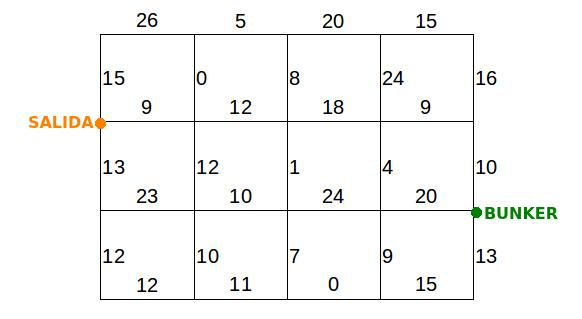
\includegraphics[scale=0.5]{imagenes/ejemplozombie.jpeg}
%	\end{center}
%	\caption{Ejemplo de ciudad para Zombieland II}\label{fig:ejzombie}
%\end{figure}
%
La solución para este ejemplo permite llegar al búnker sin perder ningún soldado, siendo el recorrido el indicado en la Figura \ref{fig:ejzombieres}.
%
%\begin{figure}[htb]
%	\begin{center}
%    		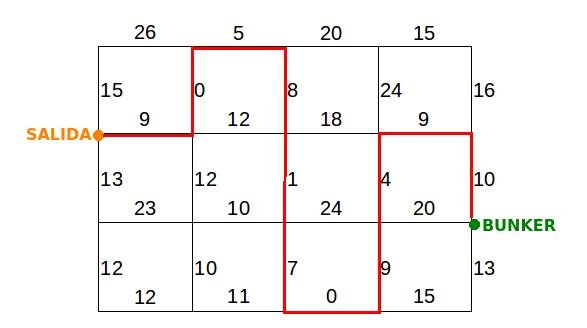
\includegraphics[scale=0.5]{imagenes/ejemplozombieres.jpeg}
%	\end{center}
%	\caption{Solución para el problema de la Figura \ref{fig:ejzombie}}\label{fig:ejzombieres}
%\end{figure}

\begin{figure}[!htb]
\minipage{0.5\textwidth}
  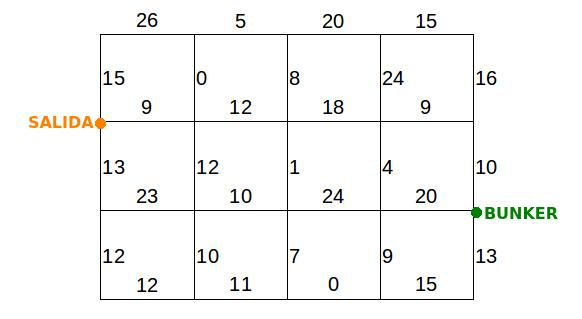
\includegraphics[scale=0.5]{imagenes/ejemplozombie.jpeg}
  \caption{Ejemplo de ciudad para Zombieland II}\label{fig:ejzombie}
\endminipage%\hspace*{3.0cm}
\minipage{0.5\textwidth}
  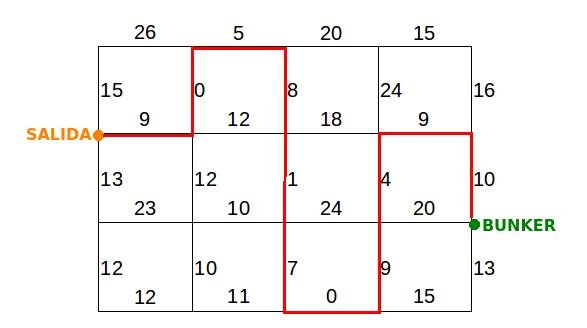
\includegraphics[scale=0.5]{imagenes/ejemplozombieres.jpeg}
  \caption{Solución para el problema de la Figura \ref{fig:ejzombie}}\label{fig:ejzombieres}
\endminipage
\end{figure}


\vspace*{0.6cm}

%\newpage
\subsection{Desarrollo de la idea y correctitud.}

\vspace*{0.3cm}



\vspace*{0.6cm}

%\newpage
%\subsection{Justificación de la resolución y demostración de correctitud.}

%\vspace*{0.3cm}



%\vspace*{0.6cm}

%\newpage
\subsection{Análisis de complejidad.}

\vspace*{0.3cm}


\vspace*{0.6cm}

%\newpage
\subsection{Experimentación y gráficos.}


\subsubsection{Test 1}

\vspace*{0.3cm}


\vspace*{0.6cm}

%\newpage
\subsubsection{Test 2}


\newpage